\documentclass[12pt]{article}
\usepackage[T1]{fontenc}
\usepackage[a4paper, total={7in, 10in}]{geometry}
\usepackage{graphicx}
\usepackage[export]{adjustbox}
\usepackage[font=normalsize,labelfont=bf]{caption}
\usepackage{caption}
\usepackage{subcaption}
\usepackage{float}
\usepackage{titling}
\usepackage{fancyhdr}
\usepackage{lipsum}

\title{Modernizacja Laboratorium Drgań}
\author{Mateusz Klisiewicz}
\newcommand{\mytitle}{MODERNIZACJA LABORATORIUM DRGAŃ MECHANICZNYCH}
\newcommand{\mysubtitle}{Plan Modelowy}
\fancyfoot{}
\fancyhead[L]{\mytitle}
\fancyhead[R]{\mysubtitle}

\fancyfoot[C]{\thepage}

\date{\today}



\renewcommand\maketitlehooka{\null\mbox{}\vfill}
\renewcommand\maketitlehookd{\vfill\null}
\renewcommand{\figurename}{Rysunek}
\graphicspath{{./tex_resources/}}
\title{\mytitle \\
  \large \mysubtitle}


\begin{document}
\pagestyle{fancy}
\maketitle
\newpage
\section*{Wstęp}
Poniższy plan ma na celu przedstawić rozwiązania dążące do ustandaryzowania, usprawnienia i ogólnej modernizacji eksperymentów wykonywanych w ramach Laboratorium Drgań Mechanicznych. W obecnej formule, istotna część zajęć często polega na rozwiązywaniu problemów technicznych i manualnej obróbce danych, przez co istota przeprowadzanego doświadczenia, a więc modelowanie i badanie zjawisk fizycznych, jest marginalizowana i niejednokrotnie pozostawiona bez wyjaśnień. \\Proponuje się zupełną zmianę podejścia do metody prowadzenia zajęć i przewartościowania wymagań stawianych studentom.
\section*{Laboratoryjna Aplikacja Komputerowa}
Proces modernizacji orientowałby się wokół aplikacji komputerowej, która w zamyśle oferowałaby zestaw nowoczesnych, atrakcyjnych wizualnie i intuicyjnych interfejsów, umożliwiających komunikację z układami elektronicznymi poszczególnych stanowisk pomiarowych.\\ W pierwszym etapie renowacji program obsługiwałby eksperymenty wykonywane na potrzeby Laboratorium Drgań Mechanicznych. Docelowo aplikacja miałaby się stać nieodłączną częścią wydziałowych przedmiotów laboratoryjnych i kluczowym elementem zajęć. 
\begin{figure}[h]
\centering
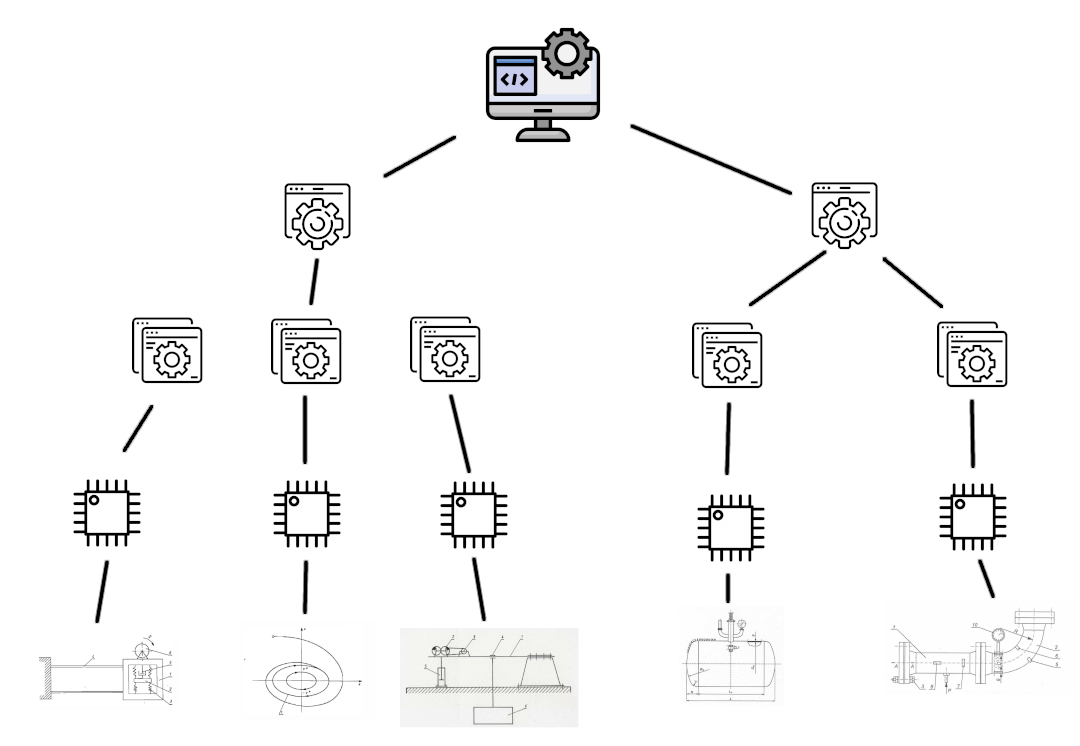
\includegraphics[width=16cm]{app_sch}
\caption{Schemat ideowy aplikacji laboratoryjnej}
\end{figure}
\newpage
\section*{Założenia}
Współcześnie, z dużą pewnością można założyć, że znacząca większość studentów posiada komputer przenośny, dlatego też planuje się tworzyć aplikację z myślą o tym, aby była ona łatwo dostępna do pobrania dla każdego. W ten sposób umożliwia się studentom prowadzenie eksperymentu z wykorzystaniem osobistego sprzętu, dzięki czemu wszelkie dane zebrane podczas zajęć zapisywane są bezpośrednio u studenta. \\
Choć jest to jeden z istotnych celów procesu modernizacji, domyślnie eksperymenty wykonywane by były na komputerach wydziałowych. Prowadzi to do wniosku, że stanowiska pomiarowe i ich elektroniczne układy powinny być projektowane z zamysłem uniwersalności i możliwości łatwej zmiany komputera zadającego parametry i zbierającego wyniki eksperymentu. Aby ten warunek mógł zostać spełniony, sugeruje się wykorzystanie interfejsu USB i standardowej komunikacji szeregowej.\\
\section*{Funkcjonalność}
Głównym założeniem programu ma być możliwość zadawania parametrów oraz zapisywania danych zebranych z czujników. Korzystając z możliwości nowoczesnych komputerów, planuje się także wbudować moduły pozwalające na modelowanie i symulacje poszczególnych eksperymentów. W ten sposób studenci dostaną możliwość szybkiej weryfikacji rozważań teoretycznych i będą mogli na bieżąco wprowadzać korekty do stworzonego przez siebie modelu, znajdując w ten sposób czynniki różniące teorię zjawiska i jego rzeczywisty przebieg. Ponadto, całkowicie automatyzując sterowanie stanowiskiem, wyklucza się podstawowe błędy pomiarowe i znacznie skraca czas trwania badania. \\
Te elementy pozwalają w istotny sposób zmienić scenariusz zajęć laboratoryjnych. Możliwość szybkiego wykonania eksperymentu pozwala wielokrotnie przeprowadzić badanie w ciągu zajęć i zwiększyć ilość analizowanych danych. Dzięki wbudowanemu symulatorowi zjawisk studenci mogą szybko przeanalizować wiele przypadków, dla różnych parametrów i warunków początkowych modelu, a następnie porównać je z uzyskanym wynikiem eksperymentu. \\
W ten sposób zajęcia laboratoryjne pokazywałyby nowoczesne metody badania układów teoretycznych i kończyłyby się precyzyjnym modelem oraz jednoznaczną przyczyną rozbieżności wyników eksperymentu i obliczeń teoretycznych.
\section*{Elementy Planu}
Wdrożenie aplikacji wymaga modyfikacji stanowisk w celu ustandaryzowania komunikacji i automatyzacji niektórych procesów. Ponadto proponuje się do rozważenia stworzenie całkowicie nowych stanowisk. Szczegóły na temat sposobu przeprowadzenia tych czynności opisano w załącznikach spisanych poniżej:\\
\begin{itemize}
\item Załącznik 1 - Aplikacja Laboratoryjna
\item Załącznik 2 - Przestrzeń (Płaszczyzna) Fazowa
\item Załącznik 3 - Dynamiczny Eliminator Drgań
\item Załącznik 4 - Sprawozdanie z Ćwiczenia "Dynamiczny Eliminator Drgań"
\item Załącznik 5 - Układ o Dwóch Stopniach Swobody
\item Załącznik 6 - Stanowisko do Badania Elementów Zawieszenia Pojazdów Jednośladowych
\end{itemize}
\end{document}